% =====================================================================
%  main.tex  --  IEEE conference paper (IEEEtran)
%  Project layout (Overleaf):
%    main.tex            this file: preamble + the order of sections
%    sections/*.tex      one file per IMRaD section, pulled in with \input
%    figures/            PDF figures (vector) and PNG (300 dpi)
%    references.bib      bibliography exported from Zotero (Better BibTeX)
% =====================================================================
\documentclass[conference]{IEEEtran}
% To switch to ACM, replace the line above with (and remove the IEEE-only blocks below):
%   \documentclass[sigconf]{acmart}        % two columns
%   \documentclass[manuscript]{acmart}     % one column, for review
% To get one column in IEEEtran, use \documentclass[journal,onecolumn]{IEEEtran}.

% ---------- encoding, fonts, typography ----------
\usepackage[T1]{fontenc}
\usepackage[utf8]{inputenc}

% ---------- citations (IEEE: numeric, sorted and compressed [1]--[3]) ----------
\usepackage{cite}

% ---------- mathematics ----------
\usepackage{amsmath,amssymb}
\usepackage{microtype}   % after amsmath, otherwise microtype cannot patch equation numbers

% ---------- tables without vertical lines ----------
\usepackage{booktabs}

% ---------- figures ----------
\usepackage{graphicx}
\graphicspath{{figures/}}

% ---------- architecture diagram (vector) ----------
\usepackage{tikz}
\usetikzlibrary{arrows.meta,positioning,fit}

% ---------- cross-references (load hyperref LAST) ----------
\usepackage[hidelinks]{hyperref}
% Names printed by \autoref
\renewcommand{\sectionautorefname}{Section}
\renewcommand{\subsectionautorefname}{Section}
\def\equationautorefname{Eq.}
\def\figureautorefname{Fig.}

\begin{document}

\title{Professional Burnout of Teachers\\
in State and Private Schools}

% TODO: add surnames and check the affiliation text
\author{\IEEEauthorblockN{Zhanat}
\IEEEauthorblockA{Narxoz University}
\and
\IEEEauthorblockN{Yergali}
\IEEEauthorblockA{Narxoz University}}

\maketitle

\begin{abstract}
Professional burnout is a recognised risk for teachers, and it may depend on the working conditions of the school.
Earlier comparisons of teachers in state and private institutions concern specific groups and report different directions of the difference.
This paper presents the protocol of a planned cross-sectional study that compares burnout of teachers in state and private schools
with the Maslach Burnout Inventory (30--40 teachers recruited from several schools of one city), together with a reproducible, containerised analysis pipeline.
The groups will be compared with Welch's $t$-test, the Mann--Whitney test and Cohen's $d$, with bootstrap confidence intervals, and the reliability of the scales will be checked with Cronbach's $\alpha$.
To show that the analysis can be repeated after every data update, we measured the pipeline on synthetic respondents:
in 120 measured runs without errors, the median latency stayed between 43.8 and 46.8\,ms for 35 to 1000 respondents,
while the throughput grew from 797 to 21\,371 respondents per second.
These results suggest that the analysis will not be a bottleneck.
The survey itself has not been conducted yet, so the research questions are left for future work, and the limitations of the design are stated explicitly.
\end{abstract}

\begin{IEEEkeywords}
teacher burnout, Maslach Burnout Inventory, state and private schools, working conditions, cross-sectional study
\end{IEEEkeywords}

\section{Introduction}\label{sec:intro}

Teaching is generally regarded as an emotionally demanding occupation, because
teachers work with many people at once and are responsible for their results.
Such conditions are associated with professional burnout, a state that Maslach
and colleagues describe through three dimensions: emotional exhaustion,
depersonalization and reduced personal accomplishment~\cite{maslach1981mbi,maslach2001job}.
A systematic review and meta-analysis of 45 articles on secondary school
teachers concluded that this group is at high risk of burnout~\cite{garciacarmona2019burnout}.

The risk is not necessarily the same in every school. The job
demands--resources model explains burnout by the balance between job demands
and the resources available to cope with them~\cite{demerouti2001jdr,bakker2007jdr};
it is flexible and can be applied to a wide range of occupations~\cite{bakker2007jdr}.
State and private schools may differ in exactly these conditions, for example
in pay, class size, administrative control and autonomy.

Comparisons of the two school types exist, but they do not give a clear
picture. In a study of special-school teachers (120 per school type), burnout was
higher in government schools than in private schools~\cite{doss2018special},
whereas in a study of 180 teachers with the MBI, teachers of English in Iranian
private language institutes reported worse burnout than their colleagues in
public schools~\cite{bahrami2019efl}. These
studies concern specific groups, they point in different directions, and the
review cited above shows that the measured prevalence depends on the
instrument~\cite{garciacarmona2019burnout}, which makes studies hard to
compare. We therefore plan a direct comparison of teachers in state and
private schools with one instrument and one analysis protocol.
% TODO (check before submission): search once more for studies of general-education teachers in our region.

We describe a planned cross-sectional study. Burnout is measured with the
Maslach Burnout Inventory in its Russian-language adaptation~\cite{vodopyanova2008burnout},
and the groups are compared with Welch's $t$-test, the Mann--Whitney test and
bootstrap confidence intervals. The study addresses three research questions:
RQ1, do burnout levels of the two groups differ (main comparison: emotional
exhaustion); RQ2, do the groups differ on each of the three scales; and RQ3,
which working conditions are associated with burnout (exploratory). The
analysis runs in a containerised pipeline, which supports reproducibility~\cite{boettiger2015docker}.

Questionnaire data may arrive in several waves, and every wave requires the
scores and tests to be recomputed. If the analysis is slow or cannot be repeated
exactly, errors and undocumented manual steps creep in. We therefore treat the
pipeline as a part of the study and check how its latency and throughput change
when the number of respondents grows.

The contributions of this work are:
\begin{itemize}
  \item a research design and analysis protocol for comparing teacher burnout
        in state and private schools, fixed before data collection;
  \item three research questions with testable hypotheses (RQ1--RQ3);
  \item an open, reproducible software pipeline for scoring the questionnaire
        and computing the statistics;
  \item a measurement of the pipeline's latency and throughput that reports
        tail percentiles~\cite{dean2013tail} with bootstrap confidence intervals.
\end{itemize}

The rest of the paper is organised as follows. \autoref{sec:method} describes
the design (\autoref{sec:design}), the instrument (\autoref{sec:instrument}), the
statistical methods (\autoref{sec:tests}), the pipeline (\autoref{sec:pipeline}) and
the measurement procedure (\autoref{sec:measure}). \autoref{sec:results} gives the
setup (\autoref{sec:setup}), the results (\autoref{sec:res}) and the discussion
(\autoref{sec:disc}), and \autoref{sec:concl} states the limitations
(\autoref{sec:limits}), concludes and outlines future work (\autoref{sec:future}).

\section{Methodology}\label{sec:method}

This section describes the planned study design, the instrument, the
statistical methods and the validation of the analysis pipeline.
All symbols are collected in \autoref{tab:notation}.

\subsection{Design and Participants}\label{sec:design}
The study is cross-sectional: every teacher fills in the questionnaire once.
Two groups are compared, teachers of state schools and teachers of private
schools. The planned sample is 30--40 teachers in total (15--20 per group),
and a group is analysed only if it contains at least 15 respondents.
Participation is voluntary and anonymous.

\subsection{Instrument and Scoring}\label{sec:instrument}
Burnout is measured with the Maslach Burnout Inventory (MBI)
\cite{maslach1981mbi,maslach2001job} in the Russian-language adaptation of
Vodopyanova and Starchenkova~\cite{vodopyanova2008burnout}. The inventory has
three scales: emotional exhaustion (EE, 9 items), depersonalization (DP, 5
items) and reduced personal accomplishment (RPA, 8 items). Each item is
answered on a scale from 0 to 6, so the scale score is the sum of its items:
\begin{equation}
  S_k = \sum_{i \in I_k} x_i, \qquad k \in \{\mathrm{EE},\mathrm{DP},\mathrm{RPA}\},
  \label{eq:scale}
\end{equation}
where $I_k$ is the set of items of scale $k$ and $x_i$ is the answer to item
$i$. The scores range from 0 to 54 for EE, from 0 to 30 for DP and from 0 to
48 for RPA. To obtain one overall burnout index, each scale is standardised
over the sample and the three values are combined:
\begin{equation}
  B = z(S_{\mathrm{EE}}) + z(S_{\mathrm{DP}}) - z(S_{\mathrm{RPA}}),
  \qquad z(S) = \frac{S - \bar{S}}{s_S},
  \label{eq:index}
\end{equation}
where $\bar{S}$ and $s_S$ are the sample mean and standard deviation of the
scale score. The sign of $z(S_{\mathrm{RPA}})$ is negative because a high
value on this scale means a high personal accomplishment, that is, less burnout.

\subsection{Reliability}\label{sec:reliability}
The internal consistency of each scale is checked with Cronbach's
$\alpha$~\cite{cronbach1951alpha}:
\begin{equation}
  \alpha = \frac{m}{m-1}\left(1 - \frac{\sum_{i=1}^{m}\sigma_i^{2}}{\sigma_{T}^{2}}\right),
  \label{eq:alpha}
\end{equation}
where $m$ is the number of items in the scale, $\sigma_i^2$ is the variance of
item $i$ and $\sigma_T^2$ is the variance of the scale score. A scale is
accepted as reliable if $\alpha \ge 0.7$.

\subsection{Group Comparison}\label{sec:tests}
The main comparison (RQ1) is the difference in emotional exhaustion between the
two groups. For group means $\bar{x}_1,\bar{x}_2$, standard deviations
$s_1,s_2$ and sizes $n_1,n_2$, we use Welch's $t$-test~\cite{welch1947t}, which
does not assume equal variances:
\begin{equation}
  t = \frac{\bar{x}_1 - \bar{x}_2}{\sqrt{s_1^{2}/n_1 + s_2^{2}/n_2}}.
  \label{eq:welch}
\end{equation}
The size of the difference is reported as Cohen's $d$:
\begin{equation}
  d = \frac{\bar{x}_1 - \bar{x}_2}{s_p},
  \qquad
  s_p = \sqrt{\frac{(n_1-1)s_1^{2} + (n_2-1)s_2^{2}}{n_1+n_2-2}}.
  \label{eq:cohen}
\end{equation}
Because of the small groups, the Mann--Whitney test~\cite{mann1947u} is
computed as a robustness check, and the uncertainty of the estimates is shown
with percentile-bootstrap confidence intervals~\cite{efron1979bootstrap}.
All tests are two-tailed with significance level $\alpha_{\mathrm{test}}=0.05$.
RQ2 repeats the comparison for each scale separately, and RQ3 is exploratory
(Spearman correlations and hierarchical regression in JASP).

\subsection{Pipeline Validation}\label{sec:pipeline}
The analysis is run by a Python pipeline in a pinned Docker image with a fixed
random seed (42). To show that the pipeline is fast enough to be re-run after
every data update, we measured it on synthetic questionnaires with
$n \in \{35,100,1000\}$ respondents. For a run $r$ with workload $n$ and
duration $\ell$, the throughput and the scaling relative to the baseline
$n_0=35$ are
\begin{equation}
  \theta = \frac{n}{\ell},
  \qquad
  S(n) = \frac{\theta(n)}{\theta(n_0)},
  \qquad
  E(n) = \frac{S(n)}{n/n_0}.
  \label{eq:speedup}
\end{equation}
Each workload was run 40 times after 10 discarded warm-up runs, and the
latency percentiles are reported with 95\,\% bootstrap intervals
($B=10\,000$ resamples). The setup is summarised in \autoref{tab:params}; the
measured latency and throughput are shown in \autoref{fig:pipeline}.
The measurements concern only the software and contain no information about
teachers.

\begin{table}[t]
  \centering
  \caption{Notation used in \autoref{eq:scale}--\autoref{eq:speedup}.}
  \label{tab:notation}
  \small
  \begin{tabular}{@{}ll@{}}
    \toprule
    Symbol & Meaning \\
    \midrule
    $S_k$ & sum score of scale $k$ (EE, DP, RPA) \\
    $z(\cdot)$ & standardised score \\
    $B$ & overall burnout index \\
    $\alpha$ & Cronbach's alpha \\
    $t$, $d$ & Welch statistic, Cohen's effect size \\
    $\theta$, $S$, $E$ & throughput, speed-up, efficiency \\
    \bottomrule
  \end{tabular}
\end{table}

\begin{table}[t]
  \centering
  \caption{Parameters of the study and of the pipeline validation.}
  \label{tab:params}
  \small
  \begin{tabular}{@{}lr@{}}
    \toprule
    Parameter & Value \\
    \midrule
    Planned sample (teachers) & 30--40 \\
    Minimum per group & 15 \\
    Significance level & 0.05 \\
    Reliability threshold $\alpha$ & 0.7 \\
    Random seed & 42 \\
    Workloads $n$ & 35, 100, 1000 \\
    Measured runs per $n$ & 40 \\
    Warm-up runs & 10 \\
    Bootstrap resamples $B$ & 10\,000 \\
    \bottomrule
  \end{tabular}
\end{table}

\begin{figure*}[t]
  \centering
  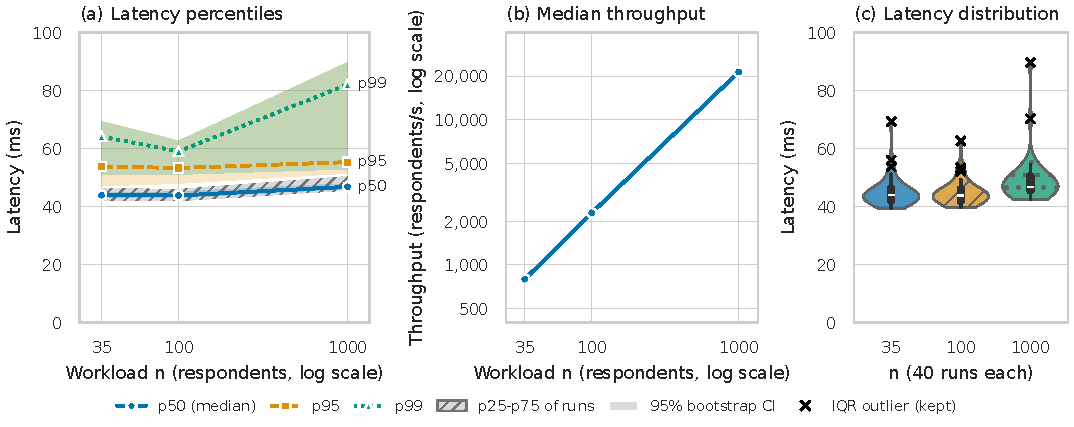
\includegraphics[width=\textwidth]{fig_combined_latency_throughput.pdf}
  \caption{Pipeline validation on synthetic data: (a)~latency percentiles,
  (b)~median throughput, (c)~distribution of run latency for
  $n=35$, $100$, $1000$ respondents (40 runs each). Bands are 95\,\%
  bootstrap intervals. Median latency stays between 43.8 and 46.8\,ms while
  throughput grows from 797 to 21\,371 respondents/s.}
  \label{fig:pipeline}
\end{figure*}

\section{Results and Discussion}\label{sec:results}

\subsection{Experimental Setup}\label{sec:setup}
The questionnaire has not been administered yet, so this draft contains no
estimates of teacher burnout; the measurements below concern only the
pipeline. They were made on ``synthetic respondents'' with the MBI structure,
on one machine inside one Docker image (Python 3.11.9), with seed 42. Ten
warm-up runs were discarded, then 40 measured runs were recorded for each
workload, interleaved in turn. Outliers (\autoref{eq:iqr}) were flagged but kept. The baseline is the
smallest workload, $n_0=35$, which equals the planned sample size
(\autoref{tab:params}). Six edge-case scenarios were also run five times each.

\subsection{Results}\label{sec:res}
\autoref{tab:results} and \autoref{fig:results} summarise the 120 measured
runs. All of them finished without an error (error rate 0\,\%), and nine runs
were flagged as outliers (3, 4 and 2 for $n=35$, 100 and 1000). The mean latency
for $n=35$ and $n=100$ (45.1 and 44.8\,ms) is higher than the median, which
indicates right-skewed run times; therefore medians and percentiles are reported. Re-running the aggregation with the
same seed gave identical statistics, which is the reproducibility check of the pipeline. \autoref{tab:edge} shows the edge cases: four invalid
inputs were rejected with an explicit message instead of being scored silently,
while two scenarios were processed. The median latency was
43.9\,ms for $n=35$, 43.8\,ms for $n=100$ and 46.8\,ms for $n=1000$. The
throughput grew almost in proportion to the workload: $S(100)=2.86$ and
$S(1000)=26.8$, that is, $E(100)=1.00$ and $E(1000)=0.94$ (\autoref{eq:speedup}).

\begin{table}[b]
  \centering
  \caption{Comparison of the workloads with the baseline $n_0=35$ (40 runs
  each). Median latency with its 95\,\% bootstrap interval; p95 and p99 in ms;
  throughput in respondents per second; speed-up $S(n)$ from \autoref{eq:speedup}.}
  \label{tab:results}
  \footnotesize
  \setlength{\tabcolsep}{3pt}
  \begin{tabular}{@{}rcccrr@{}}
    \toprule
    $n$ & Median (ms) & p95 & p99 & Resp./s & $S(n)$ \\
    \midrule
    35 (baseline) & 43.9 [43.0, 44.6] & 53.8 & 64.1 & 797 & 1.00 \\
    100  & 43.8 [43.0, 45.1] & 53.3 & 59.0 & 2\,283 & 2.86 \\
    1000 & 46.8 [46.2, 47.9] & 55.3 & 82.1 & 21\,371 & 26.8 \\
    \bottomrule
  \end{tabular}
\end{table}

\begin{table}[b]
  \centering
  \caption{Edge-case scenarios (five runs each) and the behaviour of the pipeline.}
  \label{tab:edge}
  \footnotesize
  \begin{tabular}{@{}llc@{}}
    \toprule
    Scenario & Input & Outcome \\
    \midrule
    Missing values & empty item answers & rejected \\
    Out of range & answers outside 0--6 & rejected \\
    Single group & only one school type & rejected \\
    Duplicates & repeated respondent IDs & rejected \\
    Tiny groups & very small groups & processed \\
    Straight-lining & identical answers to all items & processed \\
    \bottomrule
  \end{tabular}
\end{table}

\begin{figure*}[t]
  \centering
  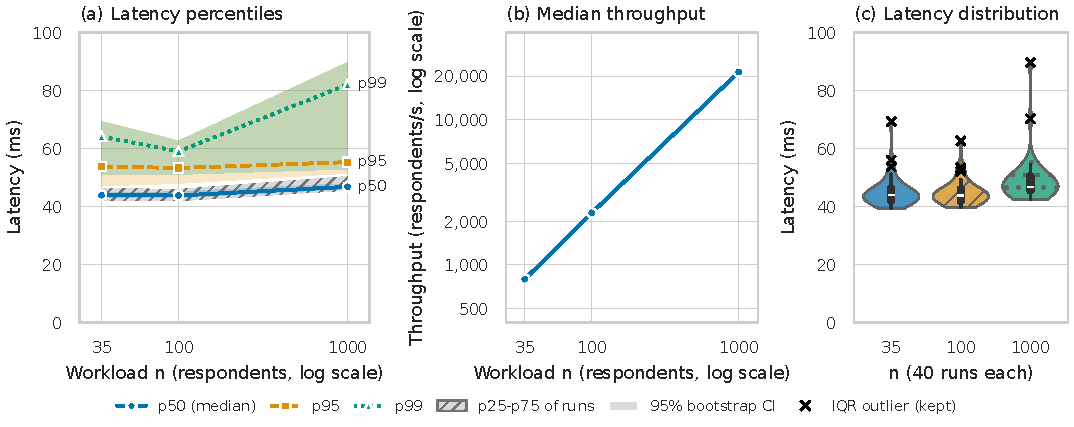
\includegraphics[width=\textwidth]{fig_combined_latency_throughput.pdf}
  \caption{Latency and throughput for $n=35$, 100 and 1000 synthetic respondents
  (40 runs each). (a)~Latency percentiles; bands are 95\,\% bootstrap intervals
  ($B=10\,000$), the hatched band is the interquartile range of the runs.
  (b)~Median throughput on logarithmic axes. (c)~Distribution of the run
  latencies; crosses mark outliers (9 of 120), which were kept.}
  \label{fig:results}
\end{figure*}

\subsection{Discussion}\label{sec:disc}
The median latency rose by only about 3\,ms (roughly 7\,\%) while the workload
grew 28-fold. This suggests that the time of a run is dominated by a fixed
overhead and not by the number of respondents. Relative to the baseline, the
larger workloads therefore cost little extra time, and since the planned sample
is of the baseline size, re-running the analysis after every data update appears
practical (the third and fourth contributions in \autoref{sec:intro}). At the measured median, a thousand repetitions of the full analysis on
1000 respondents would take roughly 47 seconds. The intervals
of the medians for $n=35$ and $n=100$ overlap, so the data do not distinguish
them, while the interval for $n=1000$ does not overlap either of them.

Tail percentiles matter for responsiveness~\cite{dean2013tail}, but here they are
the least certain values: with 40 runs, the 99th percentile is determined by the
one or two slowest runs. Its rise at $n=1000$ (82.1\,ms) is therefore a hint, not
an established effect. The analysis plan is fixed in advance (\autoref{tab:plan}), which limits the room for
analytic choices after the data have been seen. Finally, the review of teacher burnout reports that prevalence
depends on the instrument~\cite{garciacarmona2019burnout}; within the scope of our
design, this supports analysing all respondents with one instrument and one fixed protocol
(\autoref{sec:method}). Rejecting invalid input (\autoref{tab:edge}) protects later conclusions from
silent scoring errors. The measurements say nothing about burnout itself---they describe the software only.

\section{Limitations and Conclusion}\label{sec:concl}

\subsection{Limitations and Threats to Validity}\label{sec:limits}
\textit{Internal validity.} Forty runs per workload give precise medians but
imprecise tail percentiles. Interleaving, warm-up and keeping outliers limit,
but do not remove, the influence of background activity. The planned groups of
15--20 teachers are small: a power of 0.80 is reached only for large differences
($d \gtrsim 0.9$--1.1, \autoref{tab:power}), so smaller ones may be missed.
\textit{External validity.} All measurements come from one machine and one
container, so absolute times describe this environment, and the respondents are
synthetic. The teachers are recruited by convenience sampling from several
schools of one city, so the results may not generalise to other cities or to
all schools, and those who agree to take part may differ from those who decline.
\textit{Construct validity.} Latency and throughput are proxies for how practical
the pipeline is. The MBI is a self-report questionnaire, and the index $B$
(\autoref{eq:index}) is relative to the sample, so it compares the two groups
but is not an absolute level of burnout.

\subsection{Conclusion and Future Work}\label{sec:future}
We presented the protocol of a planned comparison of teacher burnout in state
and private schools and a reproducible analysis pipeline; the four contributions
of \autoref{sec:intro} are delivered except for the survey results. The survey has
not been conducted, so RQ1--RQ3 remain open and no claim about teacher burnout is
made. For RQ1, the main outcome will be the difference in emotional exhaustion with
Cohen's $d$ and its bootstrap interval; for RQ2, the same outcome for each scale;
and for RQ3, the correlations and the regression of \autoref{tab:plan}.
The measurements, however, suggest that the pipeline is fast enough for repeated
use: in 120 runs without errors, the median latency stayed between 43.8 and
46.8\,ms for 35 to 1000 respondents.

Future work has three directions: (i) to collect the data and report the results
for RQ1--RQ3; (ii) to repeat the measurements on other machines with more runs,
so that tail percentiles become reliable; and (iii) to include more schools and
regions to test whether the findings generalise.


\bibliographystyle{IEEEtran}
\bibliography{references}

\end{document}
